\chapter{Η συνεισφορά μας}

Στο κεφάλαιο αυτό αναλύεται η δική μας συνεισφορά και τα πειράματα μας. Αρχικά, περιγράφονται αναλυτικά τo διαλογικό σύστημα \en{Rasa}, καθώς και το σύστημα ενισχυτικής μάθησης \en{Vowpal Wabbit}. Έπειτα, περιγράφεται η διαδικασία που ακολουθήσαμε, καθώς και τα προβλήματα που ανέκυψαν κατά την διαδικασία. Τέλος περιγράφεται η πλήρης αρχιτεκτονική του συστήματος και η λειτουργία του.

\section{Το διαλογικό σύστημα \en{Rasa}}

Το \en{Rasa} είναι ένα πλαίσιο (\en{framework}) ανοιχτού κώδικα για την ανάπτυξη και την έκδοση εφαρμογών συνομιλίας τεχνητής νοημοσύνης. Παρέχει ένα σύνολο εργαλείων και βιβλιοθηκών που επιτρέπουν στους προγραμματιστές να δημιουργούν διαλογικούς πράκτορες, εικονικούς βοηθούς και άλλους συνομιλητές. Το \en{Rasa} έχει σχεδιαστεί για να προσφέρει ευελιξία και έλεγχο της συμπεριφοράς και των δυνατοτήτων αυτών των συστημάτων τεχνητής νοημοσύνης.

Το πλαίσιο \en{Rasa} μπορεί νοητικά να χωριστεί σε δύο κομματια. Τα κομμάτια αυτά στο παρελθόν ήταν και ξεχωριστές υπηρεσίες, αλλά πλέον όλα βρίσκονται σε ένα πακέτο: το \en{Rasa NLU (Natural Language Understanding)} υπεύθυνο για την κατανόηση φυσικής γλώσσας και το \en{Rasa Core}.

To \en{Rasa NLU} είναι υπεύθυνο για την κατανόηση των εισροών των χρηστών και την εξαγωγή σχετικών πληροφοριών από αυτές. Χρησιμοποιεί τεχνικές μηχανικής μάθησης για την επεξεργασία και την ταξινόμηση των μηνυμάτων των χρηστών, εξάγοντας οντότητες και προθέσεις.

Το \en{Rasa Core} χειρίζεται τη διαχείριση του διαλόγου και τη διαδικασία λήψης αποφάσεων. Χρησιμοποιεί ενισχυτική μάθηση για να εκπαιδεύσει μοντέλα που μπορούν να προβλέψουν την επόμενη καλύτερη ενέργεια με βάση την τρέχουσα κατάσταση της συνομιλίας. Το \en{Rasa Core} επιτρέπει στους προγραμματιστές να ορίζουν τις ροές συνομιλιών, να χειρίζονται τις απαντήσεις των χρηστών και να διαχειρίζονται το περιβάλλον και την κατάσταση.

Ένα από τα βασικά πλεονεκτήματα του \en{Rasa} είναι η ευελιξία και η δυνατότητα προσαρμογής του. Οι προγραμματιστές μπορούν να ορίσουν τα δικά τους μοντέλα γλώσσας για συγκεκριμένο τομέα, να τους εκπαιδεύσουν χρησιμοποιώντας τα δικά τους δεδομένα και να τα βελτιστοποιήσουν για να επιτύχουν καλύτερη απόδοση. Το \en{Rasa} υποστηρίζει επίσης την ενοποίηση με άλλες υπηρεσίες και πλατφόρμες, επιτρέποντας στους προγραμματιστές να συνδέουν τους διαλογικούς τους πράκτορες τους με διάφορα κανάλια, όπως ιστότοπους, εφαρμογές ανταλλαγής μηνυμάτων και φωνητικές διεπαφές.

\subsection{\en{Rasa NLU}}

Το \en{Rasa NLU} είναι το κομμάτι της εφαρμογής υπευθυνο για την κατανόηση της φυσικής γλώσσας. Το \en{Rasa} χρησιμοποιεί μια τεχνική η οποία ονομάζεται \en{DIET (Dual Intent and Entity Transformer)}, το οποίο είχε καλύτερα αποτελέσματα από \en{fine-tuning} ενός μοντέλου \en{BERT}, μετασχηματιστή που το 2020 θεωρούνταν τελευταίας τεχνολογίας. Το \en{DIET} έχει διττό ρόλο, καθώς διαχειρίζεται τόσο την αναγνώριση των προθέσεων, όσο και την εξαγωγή προθέσεων. H αρχιτεκτονική του \en{DIET} φαίνεται στο Σχήμα~\ref{fig:diet_architecture}.

Η δομή του μοντέλου είναι η εξής. Έστω ότι, για παράδειγμα, ο χρήστης λέει \en{"play ping pong"}, οταν ο πράκτορας τον ρωτήσει τι θα ήθελε να κάνει. Η πρόταση θα σπάσει σε λέξεις (\en{tokens}), και κάθε μια θα περάσει μέσα από ένα κομμάτι του δικτύου με δύο διαδρομές. Η πρώτη είναι η προ-εκπαιδευμένη διαδρομή, κάτα την οποία η λέξη περνάει μέσα από ένα προ-εκπαιδευμένο δίκτυο και επιστρέφει μια διανυσματική αναπαράσταση της λέξης. Αυτό το δίκτυο μπορεί να είναι κάποιος μετασχηματιστής για παράδειγμα. Η άλλη διαδρομή μετατρέπει πρώτα την λέξη σε μια αραιή αναπαράσταση της με βάση τις λέξεις και τα \en{n-grams} που δημιουργούνται και μετά περνάει μέσα από ένα νευρωνικό δίκτυο, κάνοντας την πράξη $g(Wx + b)$, όπου $x$ είναι η αραιή αναπαράσταση, $W$ τα βάρη του δικτύου και $b$ η κλίση (\en{bias}). Έπειτα τα δύο διανύσματα από τις δύο διαδρομές ενώνονται και περνάνε μέσα από ένα ακόμα νευρωνικό δίκτυο, το οποίο έχει ως έξοδο ένα διανυσμα 256 διαστάσεων. Τα νευρωνικά δίκτυα αυτά δεν είναι πλήρως συνδεδεμένα, αλλά έχουν αφαιρεθεί κάποιες ακμές με χρήση \en{drop-out}. Επιπλέον όλα τα νευρωνικά δίκτυα που βρίσκονται στο ίδιο επίπεδο, έχουν τα ίδια βάρη.

Πέρα από τις λέξεις, στο σύστημα εισέρχεται και το \en{\texttt{\_\_CLS\_\_} token}, το οποίο ουσιαστικά είναι η αναπαράσταση ολόκληρης της πρότασης. Αυτή η αναπαράσταση ουσιαστικά δημιουργείται είτε με την ένωση των διανυσμάτων των επιμέρους λέξεων, στο κομμάτι της δημιουργίας της αραιής αναπαράστασης είτε είναι η αναπαράσταση της πρότασης μέσα από το προ-εκπαιδευμένο δίκτυο.

Ακόμα, κατα την εκπαίδευση, μια από τις λέξεις συγκαλύπτεται με μια μάσκα, το \en{\texttt{\_\_MASK\_\_}}. Στο παράδειγμα του Σχήματος~\ref{fig:diet_architecture}, η λέξη αυτή είναι το \en{pong}. Αυτή η λέξη μετά θα πρέπει να προβλεφθεί από τον μετασχηματιστή. Αυτη η πρόβλεψη θα περάσει μετά από ενα δίκτυο διανυσματικής αναπαράστασης και θα συγκριθεί με την πραγματική λέξη. Αυτό μας δείχνει πόσο καλά το μοντέλο μας μπορεί να γενικεύσει την γλώσσα.

Ακόμα, κατά την εκπαίδευση, μια παρόμοια διαδικασία συμβαίνει μεταξύ του \en{\texttt{\_\_CLS\_\_} token} και της (γνωστής) πρόθεσης του χρήστη, καθώς στηριζόμαστε στην ιδέα ότι το \en{token}, αφού αναπαριστά ολόκληρη την πρόταση, φέρει πληροφορία σχετικά με την πρόθεση.

Τέλος, οι λέξεις αφού περάσουν μέσα από τον μετασχηματιστή, συγκρίνονται με τις πραγματικές οντότητες που αναπαριστούν μέσα σε ένα υπό συνθήκη τυχαίο πεδίο (\en{Conditional Random Field}) και υπολογίζεται μια απώλεια.

Έτσι το σύστημα ολόκληρο εκπαιδεύεται με βάση την συνολική απώλεια που προκύπτει από το σφάλμα στην αναγνώριση οντοτήτων, στην πρόβλεψη της λέξης μέσα στην πρόταση και την κατανοηση της πρόθεσης του χρήστη.





\begin{figure}
    \centering
    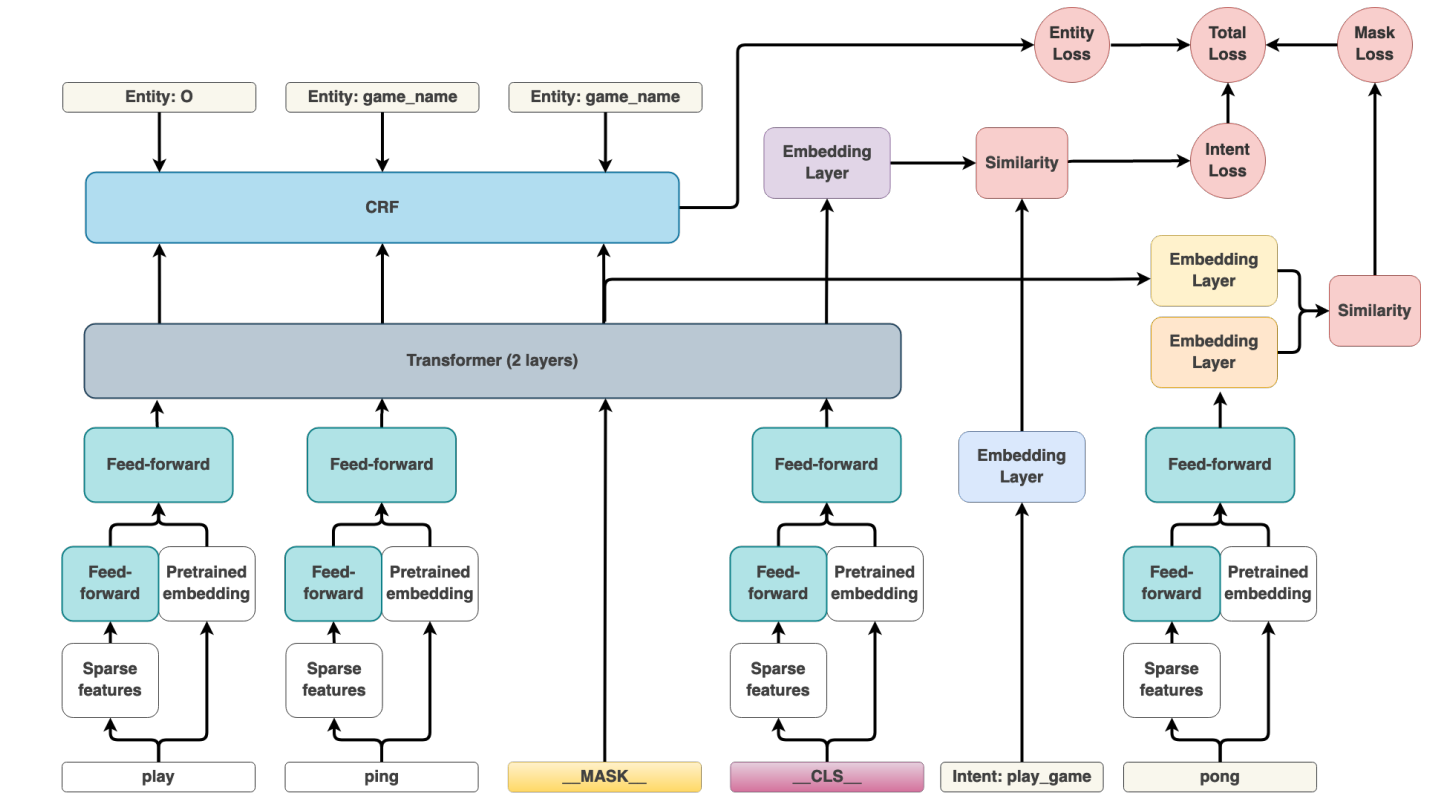
\includegraphics[width=\textwidth]{body_matter/our_work/images/DIET_architecture.png}
    \caption{Η αρχιτεκτονική του συστήματος \en{DIET}\cite{bunk2020diet}}
    \label{fig:diet_architecture}
\end{figure}

\subsection{\en{Rasa Core}}

\section{Συστάσεις μέσα στο \en{Rasa}}
